\section{匀变速直线运动的推论}
\subsection{平均速度}
平均速度的定义为:
$$\overline{v}=\cfrac{x}{t}$$
将匀变速直线运动的位移\eqref{eq:displacement}式代入平均速度公式可得:
\begin{equation}
\overline{v}=\cfrac{v+v_0}{2}
  \label{eq:average}
\end{equation}

\subsection{中间时刻的瞬时速度}

记中间时刻的瞬时速度为$v_{\frac{t}{2}}$,则由匀变速直线运动速度与时间的关系\eqref{eq:v-t}得:
\begin{align}
v_{\frac{t}{2}}-v_0 &=a\cfrac{t}{2}\\
v-v_{\frac{t}{2}} &=a\cfrac{t}{2}
\end{align}
显然上面二式的右侧相等,所以有
\begin{equation*}
v_{\frac{t}{2}}-v_0=v-v_{\frac{t}{2}}
\end{equation*}
解得:
\begin{equation}
v_{\frac{t}{2}}=\cfrac{(v+v_0)}{2}
  \label{eq:v-half-t}
\end{equation}
对比平均速度公式,此二式可以合写成:
\begin{equation}
\overline{v}=v_{\frac{t}{2}}=\cfrac{(v+v_0)}{2}
  \label{eq:v-average-half}
\end{equation}

\subsection{位移中点的瞬时速度}

位移中点的瞬时速度记为$v_{\frac{x}{2}}$,由匀变速直线运动位移与速度\eqref{eq:x-v}式可得:
\begin{align}
v^2-v_{\frac{x}{2}}^2 &=2a\cfrac{x}{2}\\
v_{\frac{x}{2}}^2-v_0^2 &=2a\cfrac{x}{2}
\end{align}
显然上面二式的右侧相等,所以有
\begin{equation*}
v^2-v_{\frac{x}{2}}^2=v_{\frac{x}{2}}^2-v_0^2
\end{equation*}
解得:
\begin{equation}
v_{\frac{x}{2}}=\sqrt{\cfrac{v^2+v_0^2}{2}}
  \label{eq:v-half-x}
\end{equation}

\subsection{$v_{\frac{t}{2}}$和$v_{\frac{x}{2}}$的大小关系}

\subsubsection{从物理角度证明}

如图\ref{fig:+t-x-middle} 画出了\CJKunderwave{匀加速直线运动}时间中点和位移中点的具体位置.

\begin{figure}[H]
  \centering
  \begin{tikzpicture}
    \draw (0,0) node [anchor=north east]{0}--(4,0) node [anchor=north west]{x};
    \draw (0,0) -- (0,0.25);
    \draw (4,0) -- (4,0.25);
    \draw (1,0) -- (1,0.25) node [anchor=south]{$v_{\frac{t}{2}}$};
    \draw (2,0) -- (2,0.25) node [anchor=south]{$v_{\frac{x}{2}}$};
    \draw (1,0) node [anchor=north]{A};
    \draw (2,0) node [anchor=north]{B};
  \end{tikzpicture}
  \caption{匀加速直线运动}
  \label{fig:+t-x-middle}
\end{figure}

由于图\ref{fig:+t-x-middle} 所示为匀加速直线运动,所以质点从A点到B 点必须\CJKunderwave{加速一段时间},所以可以得到时间中点的瞬时速度 $v_{\frac{t}{2}}$ 小于位移中点的瞬时速度 $v_{\frac{x}{2}}$

如图\ref{fig:-t-x-middle} 画出了\CJKunderwave{匀减速直线运动}时间中点和位移中点的具体位置.

\begin{figure}[H]
  \centering
  \begin{tikzpicture}
    \draw (0,0) node [anchor=north east]{0}--(4,0) node [anchor=north west]{x};
    \draw (0,0) -- (0,0.25);
    \draw (4,0) -- (4,0.25);
    \draw (3,0) -- (3,0.25) node [anchor=south]{$v_{\frac{t}{2}}$};
    \draw (2,0) -- (2,0.25) node [anchor=south]{$v_{\frac{x}{2}}$};
    \draw (2,0) node [anchor=north]{A};
    \draw (3,0) node [anchor=north]{B};
  \end{tikzpicture}
  \caption{匀减速直线运动}
  \label{fig:-t-x-middle}
\end{figure}

由于图\ref{fig:-t-x-middle} 所示为匀减速直线运动,所以质点从A点到B 点必须\CJKunderwave{减速一段时间},所以仍然可以得到时间中点的瞬时速度 $v_{\frac{t}{2}}$ 小于位移中点的瞬时速度 $v_{\frac{x}{2}}$

综合以上论述可得:

\begin{equation}
  v_{\frac{t}{2}} < v_{\frac{x}{2}} 
  \label{eq:v-t<x}
\end{equation}

\subsubsection{从数学角度证明}

对于任意的 $a>0$ ,$b>0$ 有下述均值不等式:
\[
  \sqrt{\cfrac{a^2+b^2}{2}}\geqslant\cfrac{a+b}{2}
\]

上式中,当且仅当 $a=b$ 取等号.为了保证同学们学习的连惯性,这里证明此式如下:

\begin{gather*}
 (a-b)^2 \geqslant 0\\
 a^2+b^2 -2ab \geqslant 0\\
 a^2+b^2 \geqslant 2ab
\end{gather*}

对上式,左右同时加上 $a^2+b^2$ 得

\[
2(a^2+b^2) \geqslant a^2+b^2+2ab
\]

上式右侧为完全平方式,将其写成完全平方式

\[
2(a^2+b^2) \geqslant (a+b)^2
\]

左右同时除以$4$ ,再开方,得

\[
  \sqrt{\cfrac{a^2+b^2}{2}}\geqslant\cfrac{a+b}{2}
\]

无论是匀加速还是匀减速,都有$ v\neq v_0$,如设运动的方向为正,则二个速度都大于零.所以有
\[
  \sqrt{\cfrac{v^2+v_0^2}{2}}
  >
  \cfrac{v+v_0}{2}
\]

上面正是时间中点的瞬时速度和位移中点的瞬时速度的表达式,所以有

\begin{equation*}
  v_{\frac{t}{2}} < v_{\frac{x}{2}} 
\end{equation*}

\subsection{均值不等式}
物理离不开数学,作为基本功的训练,我们在这里给出完整的均值不等式.对于任意的$a>0$和$b>0$ 前面已经证明了一组关系,即
\begin{gather}
  \cfrac{a+b}{2}\leqslant \sqrt{\frac{a^2+b^2}{2}}
  \label{eq:junzhi0}
  \intertext{同时还有关系}
  ab\leqslant \frac{a^2+b^2}{2}
  \intertext{在上式中取$\sqrt{a},\sqrt{b}$取代$a,b$的位置,得}
  \sqrt{ab}\leqslant\frac{a+b}{2}
  \label{eq:junzhi1}
  \intertext{使式\eqref{eq:junzhi1}左右同时乘以$\frac{2}{a+b}$}
  \cfrac{2\sqrt{ab}}{a+b}\leqslant 1
  \intertext{上式中左右同时乘以$\sqrt{ab}$,然后分子分母分别除以$ab$得}
  \cfrac{2}{\frac{1}{a}+\frac{1}{b}}\leqslant\sqrt{ab}
  \label{eq:junzhi2}
  \intertext{将式\eqref{eq:junzhi0},\eqref{eq:junzhi1}和\eqref{eq:junzhi2}写到一块,即构成了完整的均值不等式}
  \cfrac{2}{\frac{1}{a}+\frac{1}{b}}\leqslant\sqrt{ab}\leqslant\cfrac{a+b}{2}\leqslant\sqrt{\frac{a^2+b^2}{2}}
  \label{eq:junzhi3}
\end{gather}

\subsection{相邻相等时间段内的位移差}
设匀变速直线运动的加速度为$a$,任意相邻二段时间为$T$,此二段时间内的位移分别为$x_1$ 和$x_2$,如图\ref{fig:Delta x} 所示
\begin{figure}[H]
  \centering
  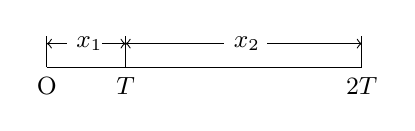
\begin{tikzpicture}
    \draw (0,0)--(4,0);
    \draw (0,0) node [anchor=north]{\small O}--(0,0.4);
    \draw (1,0) node [anchor=north]{\small $T$}--(1,0.4);
    \draw (4,0) node [anchor=north]{\small $2T$}--(4,0.4);
    \draw [<-](0,0.3)--(0.25,0.3) node [anchor=west]{\small $x_1$};
    \draw [->](0.7,0.3)--(1,0.3);
    \draw [<-](1,0.3)--(2.25,0.3) node [anchor=west]{\small $x_2$};
    \draw [->](2.8,0.3)--(4,0.3);
  \end{tikzpicture}
  \caption{等时间段内的位移差}
  \label{fig:Delta x}
\end{figure}

则有关系
\begin{equation}
x_2-x_1=aT^2
  \label{eq:Delta x}
\end{equation}
式\eqref{eq:Delta x} 不涉及初速度,一般用来处理用打点计时器所获得的纸带,因为纸带上的点是可以用毫米刻度尺来测量的,用这个方法求加速度很方便.

\subsubsection{证法一}
第一段中间时刻的瞬时速度等于第一段的平均速度,记为$v_1$,则$v_1=\cfrac{x_1}{T}$
第二段中间时刻的瞬时速度等于第二段的平均速度,记为$v_2$,则$v_2=\cfrac{x_2}{T}$
由\eqref{eq:acceleration}式得
$$a=\cfrac{v_2-v_1}{T}$$
将$v_1$和$v_2$的表达式代入得
$$a=\cfrac{x_2/T-x_1/T}{T}$$
上式分子分母同乘以$T$,然后左右同时再乘以$T^2$,移项得
$$x_2-x_1=aT^2$$
\subsubsection{证法二}
画出这段时间段内的$v-t$图象如下
\begin{figure}[H]
  \centering
  \begin{tikzpicture}
    \draw[->] (0,0) node [anchor=north]{O} -- (3.5,0) node [anchor=north]{t};
    \draw[->] (0,0)  -- (0,2.5) node [anchor=west]{v};
    \draw (0,0.5) -- (3.4,2.2);
    \draw [dotted] (1.5,0) node [anchor=north]{T}-- (1.5,1.25);
    \draw  (3,0) node [anchor=north]{2T} -- (3,2);
    \draw [dotted] (0,0.5)--(3,0.5);
    \draw [dotted] (1.5,1.25)--(3,1.25);
    \draw [pattern=north west lines] (0,0)--(1.5,0)--(1.5,1.25)--(0,0.5);
    \draw [pattern=north west lines] (1.5,1.25)--(3,1.25)--(3,2);
    \draw [pattern=north west lines] (1.5,0) rectangle (3,0.5);
    \draw (3,0.875) node [anchor=east] {\small $x_2-x_1$}; 
    \draw (0,0.5) node [anchor=east]{\small $v_0$};
    \draw [dotted] (0,1.25) node [anchor=east]{\small $v_0+aT$}--(1.5,1.25);
  \end{tikzpicture}
  \caption{相邻位移差}
  \label{fig:Delta xx}
\end{figure}

图\ref{fig:Delta xx} 中$0\sim T$ 时间段内梯形阴影面积表示位移$x_1$,$T\sim 2T$ 梯形面积表示位移$x_2$ 两面积之差就表示$x_2-x_1$,在图中所示为空白矩形的面积.矩形的长为$T$,宽为$aT$,所以其面积为$aT^2$,即
$$x_2-x_1=aT^2$$

\subsubsection{证法三}
设初速度为$v_0$,则由匀变速直线运动位移与时间的关系\eqref{eq:x-t}得
\begin{equation}
x_1=v_0T+\cfrac{1}{2}aT^2
  \label{eq:x1}
\end{equation}
\begin{equation}
x_1+x_2=v_0\cdot 2T+\cfrac{1}{2}a(2T)^2
  \label{eq:x2+x1}
\end{equation}
用式\eqref{eq:x2+x1}$-2\times$\eqref{eq:x1}得
$$x_2-x_1=aT^2$$

\subsubsection{证法四}
同证法三计算出第一段的位移,即式\eqref{eq:x1}.由匀变速直线运动速度与时间的关系\eqref{eq:v-t}得第二段的初速度为

$$v_1=v_0+aT$$

再由匀变速直线运动位移与时间关系\eqref{eq:x-t}计算第二段的位移得

\begin{equation}
x_2=(v_0+aT)\cdot T+\cfrac{1}{2}aT^2
  \label{eq:x2}
\end{equation}

用式\eqref{eq:x2} $-$ \eqref{eq:x1}得
$$x_2-x_1=aT^2$$

\subsection{逐差法求加速度}
我们首先说明为什么要用逐差法来处理问题,因为实验有误差,我们处理的原则是让误差尽可能小.一般毫米刻度尺的绝对误差是$1mm$,如图\ref{fig:rulemm}所示
\begin{figure}[H]
  \centering
  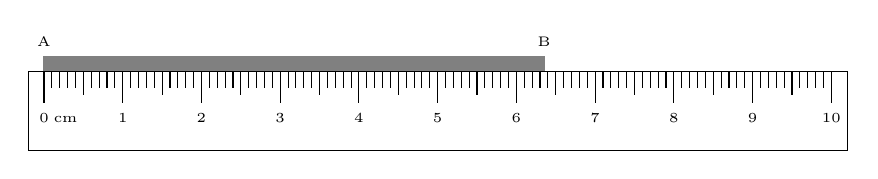
\begin{tikzpicture}
    \foreach \x in {
      0.1,0.2,0.3,0.4,0.6,0.7,0.8,0.9,
      1.1,1.2,1.3,1.4,1.6,1.7,1.8,1.9,
      2.1,2.2,2.3,2.4,2.6,2.7,2.8,2.9,
      3.1,3.2,3.3,3.4,3.6,3.7,3.8,3.9,
      4.1,4.2,4.3,4.4,4.6,4.7,4.8,4.9,
      5.1,5.2,5.3,5.4,5.6,5.7,5.8,5.9,
      6.1,6.2,6.3,6.4,6.6,6.7,6.8,6.9,
      7.1,7.2,7.3,7.4,7.6,7.7,7.8,7.9,
      8.1,8.2,8.3,8.4,8.6,8.7,8.8,8.9,
      9.1,9.2,9.3,9.4,9.6,9.7,9.8,9.9,
    }
    \draw (\x,0)--(\x,-0.2);
    \foreach \y in {0,1,2,3,4,5,6,7,8,9,10}
    \draw (\y,0)--(\y,-0.4) node [anchor=north]{\tiny \y};
    \foreach \z in {0.5,1.5,2.5,3.5,4.5,5.5,6.5,7.5,8.5,9.5}
    \draw (\z,0)--(\z,-0.3);
    \draw (-0.2,0) rectangle (10.2,-1);
    \draw (0,-0.6) node [anchor=west]{\tiny cm};
    \filldraw [color=gray] (0,0.02) rectangle (6.35,0.2);
    \draw (0,0.2) node [anchor=south]{\tiny A};
    \draw (6.35,0.2) node [anchor=south]{\tiny B};
  \end{tikzpicture}
  \caption{毫米刻度尺绝对误差}
  \label{fig:rulemm}
\end{figure}

在图\ref{fig:rulemm}中,测量一个杆的长度,使$A$ 端与零刻度线对齐,然后读$B$ 端的读数就是杆的长度.但是$B$不是完全与某一个刻度线对齐的,仔细观察不难发现它是一个介于$63mm$ 和$64mm$的数,所以坐标$x_B$ 的读数误差最大也就是$64mm-63mm=1mm$.对于一条纸带,我们在测量距离时,如图\ref{fig:zhidai}所示

\begin{figure}[H]
  \centering
  \begin{tikzpicture}
    \foreach \x in {
      0.1,0.2,0.3,0.4,0.6,0.7,0.8,0.9,
      1.1,1.2,1.3,1.4,1.6,1.7,1.8,1.9,
      2.1,2.2,2.3,2.4,2.6,2.7,2.8,2.9,
      3.1,3.2,3.3,3.4,3.6,3.7,3.8,3.9,
      4.1,4.2,4.3,4.4,4.6,4.7,4.8,4.9,
      5.1,5.2,5.3,5.4,5.6,5.7,5.8,5.9,
      6.1,6.2,6.3,6.4,6.6,6.7,6.8,6.9,
      7.1,7.2,7.3,7.4,7.6,7.7,7.8,7.9,
      8.1,8.2,8.3,8.4,8.6,8.7,8.8,8.9,
      9.1,9.2,9.3,9.4,9.6,9.7,9.8,9.9,
    }
    \draw (\x,0)--(\x,-0.2);
    \foreach \y in {0,1,2,3,4,5,6,7,8,9,10}
    \draw (\y,0)--(\y,-0.4) node [anchor=north]{\tiny \y};
    \foreach \z in {0.5,1.5,2.5,3.5,4.5,5.5,6.5,7.5,8.5,9.5}
    \draw (\z,0)--(\z,-0.3);
    \draw (-0.2,0) rectangle (10.2,-1);
    \draw (0,-0.6) node [anchor=west]{\tiny cm};
    \draw (-0.2,-0.4)--(-0.4,-0.4)--(-0.4,0.5)--(10.4,0.5)--(10.4,-0.4)--(10.2,-0.4);
    \foreach \x in {0,0.2,0.8,1.8,3.2,5,7.2,9.8}
    \filldraw [color=black] (\x , 0.05) circle [radius=1pt];
    \foreach \x in {0,0.2,0.8,1.8,3.2,5,7.2,9.8}
    \draw (\x , 0.05) node [anchor=south] {\tiny \thepointnum\stepcounter{pointnum}};
  \end{tikzpicture}
  \caption{测量纸带上点的距离}
  \label{fig:zhidai}
\end{figure}

在图\ref{fig:zhidai}中,使纸带上的计数点$0$ 与刻度尺上的零刻度对齐,然后依次读取其它点的读数,这些读数记作$x_i' \quad (i=0,1,2 \cdots)$,在纸带上标出这些读数如\ref{fig:zhidaidushu}所示

\setcounter{pointnum}{0}
\begin{figure}[H]
  \centering
  \begin{tikzpicture}
    \draw (-0.4,-0.4) rectangle (10.4,0.5); 
    \foreach \x in {0,0.2,0.8,1.8,3.2,5,7.2,9.8}
    \filldraw [color=black] (\x , 0.05) circle [radius=1pt];
    \foreach \x in {0,0.2,0.8,1.8,3.2,5,7.2,9.8}
    \draw (\x , 0.05) node [anchor=south] {\tiny \thepointnum\stepcounter{pointnum}};
    \draw (0,0)--(0,-0.8);
    \draw (0.2,0)--(0.2,-0.15);
    \draw [->,>=stealth] (0,-0.1)--(0.2,-0.1) ;
    \draw (0.2,-0.15) node {\tiny $x_1'$};
    \draw (0.8,0)--(0.8,-0.25);
    \draw [->,>=stealth] (0,-0.2)--(0.8,-0.2); 
    \draw (0.8,-0.3) node [anchor=south east] {\tiny $x_2'$};
    \draw (1.8,0)--(1.8,-0.35);
    \draw [->,>=stealth] (0,-0.3)--(1.8,-0.3) node [anchor=south east] {\tiny $x_3'$};
    \draw (3.2,0)--(3.2,-0.45);
    \draw [->,>=stealth] (0,-0.4)--(3.2,-0.4)node [anchor=south east] {\tiny $x_4'$};
    \draw (5,0)--(5,-0.55);
    \draw [->,>=stealth] (0,-0.5)--(5,-0.5)node [anchor=south east] {\tiny $x_5'$};
    \draw (7.2,0)--(7.2,-0.65);
    \draw [->,>=stealth] (0,-0.6)--(7.2,-0.6)node [anchor=south east] {\tiny $x_6'$};
    \draw (9.8,0)--(9.8,-0.75);
    \draw [->,>=stealth] (0,-0.7)--(9.8,-0.7)node [anchor=south east] {\tiny $x_7'$};
  \end{tikzpicture}
  \caption{计数点的读数标记}
  \label{fig:zhidaidushu}
\end{figure}

我们以不带撇号的坐标表示两点间的距离,如图\ref{fig:zhidaijvli}所示

\setcounter{pointnum}{0}
\begin{figure}[H]
  \centering
  \begin{tikzpicture}
    \draw (-0.4,-0.4) rectangle (10.4,0.5); 
    \foreach \x in {0,0.2,0.8,1.8,3.2,5,7.2,9.8}
    \filldraw [color=black] (\x , 0.05) circle [radius=1pt];
    \foreach \x in {0,0.2,0.8,1.8,3.2,5,7.2,9.8}
    \draw (\x , 0.05) node [anchor=south] {\tiny \thepointnum\stepcounter{pointnum}};
    \draw [<-,>=stealth] (0.2,0.05)--(0.4,0.05);
    \draw (0.5,0.05) node {\tiny $x_2$};
    \draw [->,>=stealth] (0.6,0.05)--(0.8,0.05);
    \draw [<-,>=stealth] (0.8,0.05)--(1.15,0.05);
    \draw (1.3,0.05) node {\tiny $x_3$};
    \draw [->,>=stealth] (1.45,0.05)--(1.8,0.05);
    \draw [<-,>=stealth] (1.8,0.05)--(2.35,0.05);
    \draw (2.5,0.05) node {\tiny $x_4$};
    \draw [->,>=stealth] (2.65,0.05)--(3.2,0.05);
    \draw [<-,>=stealth] (3.2,0.05)--(3.95,0.05);
    \draw (4.1,0.05) node {\tiny $x_5$};
    \draw [->,>=stealth] (4.25,0.05)--(5,0.05);
    \draw [<-,>=stealth] (5,0.05)--(5.95,0.05);
    \draw (6.1,0.05) node {\tiny $x_6$};
    \draw [->,>=stealth] (6.25,0.05)--(7.2,0.05);
    \draw [<-,>=stealth] (7.2,0.05)--(8.35,0.05);
    \draw (8.5,0.05) node {\tiny $x_7$};
    \draw [->,>=stealth] (8.65,0.05)--(9.8,0.05);
  \end{tikzpicture}
  \caption{计数点的距离标记}
  \label{fig:zhidaijvli}
\end{figure}

由于我在这里作图是按照标准的$1:3:5:7:9:11$ 完成的,第一段的距离太小,为了防止第一段看不清楚,所以在第一段上没有标出$x_1$,同时由图 \ref{fig:zhidaidushu}和图\ref{fig:zhidaijvli}对比可知两种表示方法的关系为

\begin{equation}
  x_i=x_i'-x_{i-1}' \qquad (i=1,2,3 \cdots)
  \label{eq:dushujvli}
\end{equation}

下面我们讨论加速度的计算,由$x_2$ 和$x_1$ 我们可以计算加速度,如下
\begin{gather}
  x_2-x_1=a_1T^2
  \intertext{经过简单计算可得}
  a_1=\frac{x_2-x_1}{T^2}
  \intertext{同理也可以得到加速度}
  a_2=\frac{x_3-x_2}{T^2}\\
  a_3=\frac{x_4-x_3}{T^2}\\
  a_4=\frac{x_5-x_4}{T^2}
  \intertext{由于在$a_1$的分子部分需要三个坐标来确定这个差,所以它的误差为$3mm$,$a_2$和$a_3$需要四个坐标来确定分子部分的差,所以其误差为$4mm$,但$T$是相同的,下面我们将这四个加速度取几何平均,则得到}
  a_{1234}=\frac{1}{4}(a_1+a_2+a_3+a_4)=\frac{x_5-x_1}{4T^2}
  \intertext{上面这个平均加速度,其分子部分需要三个坐标确定,但是分子上需要除以$4$,所以它的误差为$3mm/4=0.75mm$,同理我们可以得到$a_{2345}$等类似的平均值,如下}
  a_{2345}=\frac{1}{4}(a_2+a_3+a_4+a_5)=\frac{x_6-x_2}{4T^2}\\
  a_{3456}=\frac{1}{4}(a_3+a_4+a_5+a_6)=\frac{x_7-x_3}{4T^2}
  \intertext{上面的$a_{2345}$和$a_{3456}$的分子部分需要4个坐标确定,所以它们的误差是$4mm/4=1mm$,但是如果再取一次平均,如下}
  a=\frac{1}{3}(a_{1234}+a_{2345}+a_{3456})=\frac{(x_5+x_6+x_7)-(x_1+x_2+x_3)}{3\times 4T^2}
  \intertext{上式分子部分等于$x_7'-x_4'-x_3'$,用到了三个读数,但是分母上需要除以$12$ 所以它的误差是$3mm/12=0.25mm$,所以最后这个结果误差是最小的,为我们所采纳,这就是逐差法公式.下面我们总结写出加速度的方法,分母上的这个数值可以这样来确定:分子中的括号中有$3$个数值,同时每个数值的下标差相同(比如$5-1=4$,$6-2=4$,$7-3=4$),分母上的这个数值就是$3\times4=12$,同理我们可以写出$6$段和$9$段的计算公式如下}
  a=\frac{(x_4+x_5+x_6)-(x_1+x_2+x_3)}{3\times3 T^2}\\
  a=\frac{(x_6+x_7+x_8+x_9)-(x_1+x_2+x_3+x_4)}{4\times5 T^2}
  \intertext{有许多人为了方便记住逐差法的公式,在偶数段时将纸带一分为二,比如$6$段时,可以写作}
  a=\frac{(x_4+x_5+x_6)-(x_1+x_2+x_3)}{(3T)^2}
  \intertext{这可以理解为时间间隔为$3T$ 的两大段,使用$\Delta x=aT^2$ 一步写出,但是在遇到奇数段(比如$7$段)的时候就会遇到麻烦,如果按这个逻辑,可以选用前$6$段或者后$6$段,这样写出的公式误差是$3mm/9=0.33mm$,而按逐差法写出的公式是\CJKunderwave{去掉中间一段}这样计算的结果误差为$3mm/12=0.25mm$,显然\CJKunderwave{去掉中间一段}才能得到更精确的答案.}
  \notag
\end{gather}

\subsection{初速度为零的比例关系}

匀变速直线运动的比例关系共有两大组,其一按\CJKunderwave{时间等分},其二按\CJKunderwave{位移等分}.

\subsubsection{按时间等分}

时间每隔 $T$ 分一份,则 $T$ ,$2T$,$3T$,$\cdots$ 等时刻对应的速度分别为 $v_1$,$v_2$,$v_3$,$\cdots$

由\eqref{eq:v-t} 式,可得
\[
  v_n=a\cdot nT
\]

所以有

\begin{equation}
  v_1 : v_2 :v_3 : \cdots : v_n = 1 : 2 : 3 :\cdots  : n 
  \label{eq:v-frac}
\end{equation}

从0时刻开始,$0\sim T$, $0\sim 2T$, $0\sim 3T $ ,$ \cdots$ 等时间间隔内对应的位移分别记为 $x_1$ , $x_2$ , $x_3$, $\cdots$

由 \eqref{eq:x-t} 式,可得

\[
  x_n=\cfrac{1}{2}a\cdot (nT)^2
\]

所以有

\begin{equation}
  x_1 : x_2 :x_3 : \cdots : x_n = 1^2 : 2^2 : 3^2 :\cdots  : n^2 
  \label{eq:x-frac}
\end{equation}

第 $T$ ,第 $2T$ ,第 $3T$ , $\cdots$ ,第 $nT$ 时间间隔内对应的位移分别记为
$\Delta x_1$ , $\Delta x_2$ , $\Delta x_3$, $\cdots$ , $\Delta x_n$

由$x_n$ 与 $n$ 的关系可得
\[
  \Delta x_n =x_n-x_{n-1}=(2n-1)\cdot \cfrac{1}{2}aT^2
\]

所以有

\begin{equation}
 \Delta x_1 :\Delta x_2 :\Delta x_3 : \cdots :\Delta x_n 
 = 1 : 3 : 5 :\cdots  : (2n-1)
  \label{eq:Delta x-frac}
\end{equation}

\subsubsection{按位移等分}

位移每隔$L$ 分一份,记 $L$ ,$2L$ , $3L$ , $\cdots $ , $nL$ 等位置时,质点的速度分别为 $v_1$ , $v_2$ ,$v_3$ , $\cdots$ , $v_n$ 

由\eqref{eq:x-v} 式,可得

\[v_n^2-0=2ax_n\]

代入 $x_n=nL$ 解得
\[
  v_n=\sqrt{n\cdot 2aL}
\]

所以有

\begin{equation}
  v_1 : v_2 : v_3 : \cdots : v_n =\sqrt{1} : \sqrt{2} :\sqrt{3} :\cdots :\sqrt{n} 
  \label{eq:v-x-frac}
\end{equation}

记质点到达 $L$ ,$2L$ , $3L$ , $\cdots $ , $nL$ 等位置时,需要的时间分别为 $t_1$ , $t_2$ ,$t_3$ , $\cdots$ , $t_n$ 

由\eqref{eq:x-t} 式,可得
\[x_n=\cfrac{1}{2}at_n^2\]

代入 $x_n=nL$ 解得
\[
  t_n=\sqrt{\cfrac{2nL}{a}}
\]

所以有

\begin{equation}
  t_1 : t_2 : t_3 : \cdots : t_n =\sqrt{1} : \sqrt{2} :\sqrt{3} :\cdots :\sqrt{n} 
  \label{eq:t-x-frac}
\end{equation}

记质点经过第一个 $L$ ,第二个$L$, 第三个$ L$ , $\cdots$ ,第$n$ 个 $L$ 等位移时,需要的时间分别为$\Delta t_1$ , $\Delta t_2$ ,$\Delta t_3$ , $\cdots$ , $\Delta t_n$ 

由$t_n$ 的表达式可得
\[
  \Delta t_n = t_n - t_{n-1}=(\sqrt{n}-\sqrt{n-1})\sqrt{\cfrac{2L}{a}}
\]

所以有

\begin{equation}
  \Delta t_1 : \Delta t_2 : \Delta t_3 : \cdots : \Delta t_n =\sqrt{1} : (\sqrt{2}-\sqrt{1}) :(\sqrt{3}-\sqrt{2}) :\cdots :(\sqrt{n}-\sqrt{n-1} )
  \label{eq:Delta t-x-frac}
\end{equation}
